\documentclass[12pt]{article}

\usepackage{amsmath,amsthm,amsfonts,amssymb,amsxtra}
\usepackage{pgf,tikz}
\usetikzlibrary{arrows}
\renewcommand{\theenumi}{(\alph{enumi})} 
\renewcommand{\labelenumi}{\theenumi}

\pagestyle{empty}
\setlength{\textwidth}{7in}
\setlength{\oddsidemargin}{-0.5in}
\setlength{\topmargin}{-1.0in}
\setlength{\textheight}{9.5in}

\theoremstyle{definition}
\newtheorem{problem}{Problem}

\begin{document}

\noindent{\large\bf MATH 242}\hfill{\large\bf Test \#1}\hfill{\large\bf Fall 2018}\hfill{\large\bf Page 1/7}\hrule

\bigskip
\begin{center}
  \begin{tabular}{|ll|}
    \hline & \cr
    {\bf Name: } & \makebox[12cm]{\hrulefill}\cr & \cr
    {\bf VIP ID:} & \makebox[12cm]{\hrulefill}\cr & \cr
    \hline
  \end{tabular}
\end{center}
\begin{itemize}
\item Write your name and VIP ID in the space provided above.
\item The test has seven (7) pages, including this one.
\item Six of those pages contain one or several problems, for a total worth of 25 points.
\item Mark in the table below the four pages that you want me to grade.  I will not grade any page that is not marked in
  the table below.  If you mark more than four pages, I will only grade the first four.
\item Credit for each problem is given at the right of each problem number.
\item For each problem, enter your answer in the box(es) provided.
\item Show sufficient work to justify all answers unless otherwise stated in the problem.  Correct answers with
  inconsistent work may not be given credit.
\item No books or notes are allowed.  You may use a graphing calculator with no Computer Algebra System.
\end{itemize}
\hrule

\begin{center}
  \begin{tikzpicture}
    \draw (0,0) node[scale=0.75]{%
      \begin{tabular}{|c|c|c|c|}
        \hline
        &&&\cr
            {\large\bf Page} & {\large\bf Max} & {\large\bf Grade it?} & {\large\bf Points} \cr
        &&&\cr
            \hline
        &&&\cr
            {\Large 2} & \Large 25 & & \cr
        &&&\cr
            \hline
        &&&\cr
            {\Large 3} & \Large 25 & & \cr
        &&&\cr
            \hline
        &&&\cr
            {\Large 4} & \Large 25 & & \cr
        &&&\cr
            \hline
        &&&\cr
            {\Large 5} & \Large 25 & & \cr
        &&&\cr
            \hline
        &&&\cr
            {\Large 6} & \Large 25 & & \cr
        &&&\cr
            \hline
        &&&\cr
            {\Large 7} & \Large 25 & & \cr
        &&&\cr
            \hline\hline
        &&&\cr
            {\large\bf Total} & \Large 100 & & \cr
        &&&\cr
            \hline
      \end{tabular}};
  \end{tikzpicture}
\end{center}
\newpage

%%%%%%%%%%%%%%%%%%%%%%%%%%%%%%%%%%%%% Page 2
\noindent{\large\bf MATH 242}\hfill{\large\bf Test \#1}\hfill{\large\bf Fall 2018}\hfill{\large\bf Page 2/7}\hrule 

\bigskip

\begin{problem}[25 pts]
  Consider the following differential equation:
  \begin{equation*}
    y' = x^2 (3-y)
  \end{equation*}
  \begin{enumerate}
  \item \textbf{[5pts]} What kind of equation is it?
    \begin{flushright}
      \begin{tikzpicture}
        \draw (0cm,1.4cm) rectangle (9cm,2.4cm);
        \draw (-1.75cm, 1.9cm) node {This equation is };
      \end{tikzpicture}
    \end{flushright}
  \item \textbf{[5 pts]} Find an \emph{implicit form} of its \textbf{general solution}.
    \vspace{4.25cm}
    \begin{flushright}
      \begin{tikzpicture}
        \draw (0cm,1.4cm) rectangle (7cm,2.8cm);
      \end{tikzpicture}
    \end{flushright}  
  \item \textbf{[5 pts]} Find a \emph{particular solution} that solves the following \textbf{initial value problem}.
    \begin{equation*}
      y' = x^2 (3-y), \quad y(0) = 3-e
    \end{equation*}
    \begin{flushright}
      \begin{tikzpicture}
        \draw (-0.5cm,2.1cm) node {$y=$};
        \draw (0cm,1.4cm) rectangle (5cm,2.8cm);
      \end{tikzpicture}
    \end{flushright}
  \item \textbf{[5 pts]} Are there any \textbf{singular solutions}?  Find at least one.
    \begin{flushright}
      \begin{tikzpicture}
        \draw (-0.5cm,2.1cm) node {$y=$};
        \draw (0cm,1.4cm) rectangle (5cm,2.8cm);
      \end{tikzpicture}
    \end{flushright}
  \item \textbf{[5 pts]} Find an explicit \emph{particular solution} that solves this other \textbf{initial value problem}.
    \begin{equation*}
      y' = x^2 (3-y), \quad y(0) = 3
    \end{equation*}
    \begin{flushright}
      \begin{tikzpicture}
        \draw (-0.5cm,2.1cm) node {$y=$};
        \draw (0cm,1.4cm) rectangle (5cm,2.8cm);
      \end{tikzpicture}
    \end{flushright}
  \end{enumerate}
\end{problem}
\newpage

%%%%%%%%%%%%%%%%%%%%%%%%%%%%%%%%%%%%% Page 3
\noindent{\large\bf MATH 242}\hfill{\large\bf Test \#1}\hfill{\large\bf Fall 2018}\hfill{\large\bf Page 3/7}\hrule

\bigskip
\begin{problem}[10 pts---all or nothing]
  Which of the following is the slope field of the following differential equation?
  \begin{equation*}
    y' = x^2 -x-2
  \end{equation*}
  \noindent (You do not need to show work)
  \begin{center}
    \begin{tabular}{cc}
      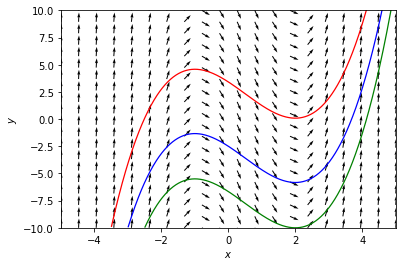
\includegraphics[width=0.5\linewidth]{quiver1.png} & 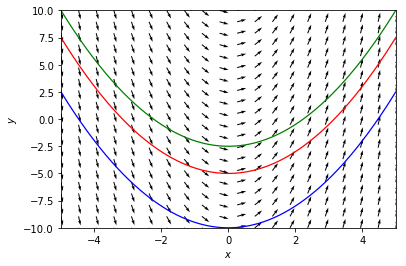
\includegraphics[width=0.5\linewidth]{quiver2.png}
    \end{tabular}
  \end{center}
\end{problem}
\hrule

\begin{problem}[15 pts]
  Use Euler's method with a step size $h=0.5$ to obtain a numerical approximation of the following \textbf{initial value problem}:
  \begin{equation*}
    y' = xy^2, \quad y(0)=1
  \end{equation*}
  \vspace{5cm}
  \begin{flushright}
    \begin{tabular}{|c||c|c|c|}
      \hline
      $n$ & $x_n$ & $y_n$ & $f(x_n, y_n)$ \\ 
      \hline \hline
          &&& \\
      $0$ & \hspace{0.5cm} & \hspace{1cm} & \hspace{3cm} \\
          &&& \\ \hline
          &&& \\
      $1$ &&& \\
          &&& \\ \hline
          &&& \\
      $2$ &&& \\
          &&& \\ \hline
          &&& \\      
      $3$ &&& \\
          &&& \\ \hline      
    \end{tabular}
  \end{flushright}
\end{problem}
\newpage

%%%%%%%%%%%%%%%%%%%%%%%%%%%%%%%%%%%%% Page 4
\noindent{\large\bf MATH 242}\hfill{\large\bf Test \#1}\hfill{\large\bf Fall 2018}\hfill{\large\bf Page 4/7}\hrule

\bigskip

\begin{problem}[10 pts]
  Solve the following differential equation.  (Assume $x>0$)
  \begin{equation*}
    \big( x^3 + \tfrac{y}{x} \big) + \big( y^2 + \ln x \big) y' = 0
  \end{equation*}

  \vspace{6.5cm}
  \begin{flushright}
    \begin{tikzpicture}
      \draw (0cm,-0.2cm) rectangle (9cm,1.2cm);
    \end{tikzpicture}
  \end{flushright}
\end{problem}
\hrule

\begin{problem}[15 pts]
  Solve the following differential equation:
  \begin{equation*}
    \frac{dy}{dx} = \frac{y}{x} + e^{y/x}
  \end{equation*}

  \vspace{7.5cm}
  \begin{flushright}
    \begin{tikzpicture}
      \draw (0cm,-0.2cm) rectangle (9cm,1.2cm);
    \end{tikzpicture}
  \end{flushright}
\end{problem}
\newpage

%%%%%%%%%%%%%%%%%%%%%%%%%%%%%%%%%%%%% Page 4
\noindent{\large\bf MATH 242}\hfill{\large\bf Test \#1}\hfill{\large\bf Fall 2018}\hfill{\large\bf Page 5/7}\hrule

\bigskip

\begin{problem}[25 pts]
  Solve the following differential equation. (Assume $x>0$)
  \begin{equation*}
    xy' + y = xy^2 \ln x
  \end{equation*}

  \vspace{18cm}
  \begin{flushright}
    \begin{tikzpicture}
      \draw (0cm,-0.2cm) rectangle (9cm,1.2cm);
    \end{tikzpicture}
  \end{flushright}
\end{problem}
\newpage

%%%%%%%%%%%%%%%%%%%%%%%%%%%%%%%%%%%%% Page 4
\noindent{\large\bf MATH 242}\hfill{\large\bf Test \#1}\hfill{\large\bf Fall 2018}\hfill{\large\bf Page 6/7}\hrule

\bigskip

\begin{problem}[10 pts]
  Find a general solution to the following differential equation.
  \begin{equation*}
    y''-4y'+4y=3e^{2x}
  \end{equation*}

  \vspace{6cm}
  \begin{flushright}
    \begin{tikzpicture}
      \draw (0cm,-0.2cm) rectangle (9cm,1.2cm);
    \end{tikzpicture}
  \end{flushright}
\end{problem}
\hrule

\begin{problem}[15 pts]
  Solve the following differential equation. (Assume $y,y'>0$)
  \begin{equation*}
    y y'' + \big(y'\big)^2=0
  \end{equation*}

  \vspace{10cm}
  \begin{flushright}
    \begin{tikzpicture}
      \draw (0cm,-0.2cm) rectangle (9cm,1.2cm);
    \end{tikzpicture}
  \end{flushright}
\end{problem}
\newpage

%%%%%%%%%%%%%%%%%%%%%%%%%%%%%%%%%%%%% Page 4
\noindent{\large\bf MATH 242}\hfill{\large\bf Test \#1}\hfill{\large\bf Fall 2018}\hfill{\large\bf Page 7/7}\hrule

\bigskip

\begin{problem}[25 pts]
  Given the differential equation $x^2y''-2xy'+2y=0$,
  \begin{enumerate}
  \item \textbf{[10 pts]} Verify that the functions $y_1=x$ and $y_2 = x^2$ are particular solutions.
  \item \textbf{[5 pts]} Compute the Wronskian of $y_1$ and $y_2$.  Indicate where we are guaranteed a solution of the
    differential equation in the form $y=Ay_1 + By_2$.
  \item \textbf{[10 pts]} Find a particular solution if initial conditions are given by $y(1)=3, y'(1)=1$.

  \end{enumerate}
\end{problem}

\end{document}
